%this file is the analysis report of POO project
%a % comment anything after % until the end of the line
%minimum references to begin our article
\documentclass[12pt]{article}

\usepackage[french]{babel}
\usepackage[utf8]{inputenc}
\usepackage[T1]{fontenc}
\usepackage{graphicx}
\usepackage{fancyhdr}
\usepackage{hyperref}
\usepackage{float}
\usepackage{amsmath}
%\usepackage[margin=1in]{geometry}
%\usepackage{indentfirst}
%\usepackage{titlesec}

\newcommand{\sectionbreak}{\clearpage}
\pagestyle{fancy}
%\cfoot{Rapport de présentation projet POO}
% the last extension makes it possible to add images
%presentation of the document
\title{Projet Modéliation et Programmation Orientée Objet\break Rapport d'analyse et de conception logicielle}
\author{Julien \textsc{Bouvet}, Mikail \textsc{Demirdelen} \\}
\date{08/11/2014}
\setlength\parindent{15pt}
\begin{document}
\maketitle
\newpage
\newpage
%to add a table of contents
\tableofcontents
\newpage
\section{Introduction}

Dans le cadre du Projet Programmation et Modélisation Orientée-Objet, nous allons modéliser un réaliser un jeu de stratégie au tour par tour. \newline \newline
Le principe de ce projet est d'avoir une première aproche de la programmation et modélisation orientée-objet à travers un logiciel relativement complexe. Nous allons passer par différentes phases de conception.
\begin{itemize}
  \item Analyse du jeu : Nous devrons comprendre et assimiler le fonctionnement du jeu afin de concevoir son fonctionnement logiciel. De plus, nous allons devoir en détailler les règles.
  \item Analyse de la structure du logiciel :  A l'aide de différents diagrammes, nous allons pouvoir définir conceptuellement plusieurs classes, leurs différentes relations et interactions. De plus, nous devrons utiliser des patrons de conception pour rendre plus générique la modélation de notre logiciel.
  \item Implémentation du jeu : Nous allons développer concrètement le jeu dans les langage C\# et C++ , nous permettant d'appliquer les principes de programmation orientée objet.
\end{itemize}

\newpage
\section{Présentation du jeu}
Le but du projet est de développer est un jeu de stratégie au tour par tour. Chaque joueur contrôle un peuple et doit gérer des unités sur une carte afin d'obtenir le plus de points possible après un certain nombre de tours de jeu. Détaillons-en les différentes spécificités.
\subsection{Les peuples}
Il existe trois peuples : les Elfs, les Orcs et les Nains, dont les caractéristiques influent sur les différentes stratégies de jeu. Un peuple ne peut être choisi que par un seul joueur et a des bonus/malus en fonction des conditions environnementales ou des actions effectuées par les unités. Par exemple, le coût d'un déplacement en forêt, pour un elf, est divisé par deux. Autre exemple, un orc qui tue une unité au combat gagne un point bonus permanent.

\subsection{La Carte du monde}
La carte du monde se compose de cases hexagonales dont il existe différents types : Désert, Montagne, Forêt et Plaine. Ces différents terrains interagissent avec les unités en fonction du peuple auquel elles appartiennent, permettant ainsi de développer plusieurs stratégies.

\subsection{Types de cartes}
Il existe 3 types de cartes :
\begin{itemize}
  \item Démo : 2 joueurs, 6 cases x 6 cases, 4 unités par joueur.
  \item Petite : 2 joueurs, 10 cases x 10 cases, 6 unités par joueur.
  \item Normale :  2 joueurs, 14 cases x 14 cases, 8 unités par joueur.
\end{itemize}
Le nombre de case est multiple de 4, puisque le terrain comporte autant de cases de chaque type disponible.
\subsection{Les Combats}
Pour qu'une unité attaque une autre unité, ils faut qu'elles se trouvent sur des cases adjacentes. Lorsqu'une unité attaque une case contenant plusieurs unités, la meilleure unité défensive est choisie. Chaque combat calcule les probabilités de perte d'une vie de l'attaquant selon la formule suivante :
\bigskip
\begin{minipage}[b]{1\linewidth}
\centering
\begin{equation*}
P = \frac{1 - (A - D)}{2} + 0,5
\end{equation*}
\medskip
\textit{Calcul de la probabilité pour l'attaquant de perdre une vie}
\end{minipage}%

\bigskip
\begin{itemize}
  \item \ensuremath{P}: probabilité de perte d'une vie de l'attaquant
  \item \ensuremath{A}: points d'attaque de l'unité offensive
  \item \ensuremath{D}: points de défense de l'unité attaquée.
\end{itemize}
\bigskip

Par exemple, prenons une unité ayant 3 points d'attaque déclenche un combat contre une autre unité ayant 4 points de défense, selon cette formule, il aura 62.5\% de chances de perdre une vie.\\

De plus, les points de vie rentrent en compte dans le calcul des probabilités : on pondère le nombre de points d'attaque par le pourcentage de points de vie restants. Une unité avec 4 points d'attaque de base et 50\% de sa vie se retrouvera, au final, avec 2 points d'attaque.\\\\
Enfin, lorsqu'un attaquant gagne le combat, il se déplace automatiquement sur la case du défenseur si elle est vide. Cela lui coûte un point de déplacement quel que soit le type de la case ou de l'unité.

\subsection{Le jeu}
\subsubsection{Début du jeu}
Chaque joueur commence la partie en sélectionnant son peuple (le choix du premier joueur est fait aléatoirement). Pour commencer, les unités du peuples sont placées sur la même case. Les joueurs jouent tour à tour sur le même ordinateur.
\subsubsection{Déroulement d'un tour}
Lorsqu'un joueur peut jouer, il peut choisir de déplacer ses unités ou d'attaquer une unité adverse s'il est à portée. Dans tous les cas, il devra lui rester assez de point de déplacement.

Lorsqu'un joueur a fini son tour, il clique sur le bouton Fin de tour, ce qui permet à l'autre de commencer son tour.

\newpage
\section{Présentation du logiciel}

\subsection{Architecture générale}
Notre première analyse porta sur l'architecture générale du logiciel. Nous avons ainsi conçu un diagramme de classe correspondant à notre vision du jeu, représenté à la figure \ref{classe}.

\begin{figure}[!h] 
\centerline{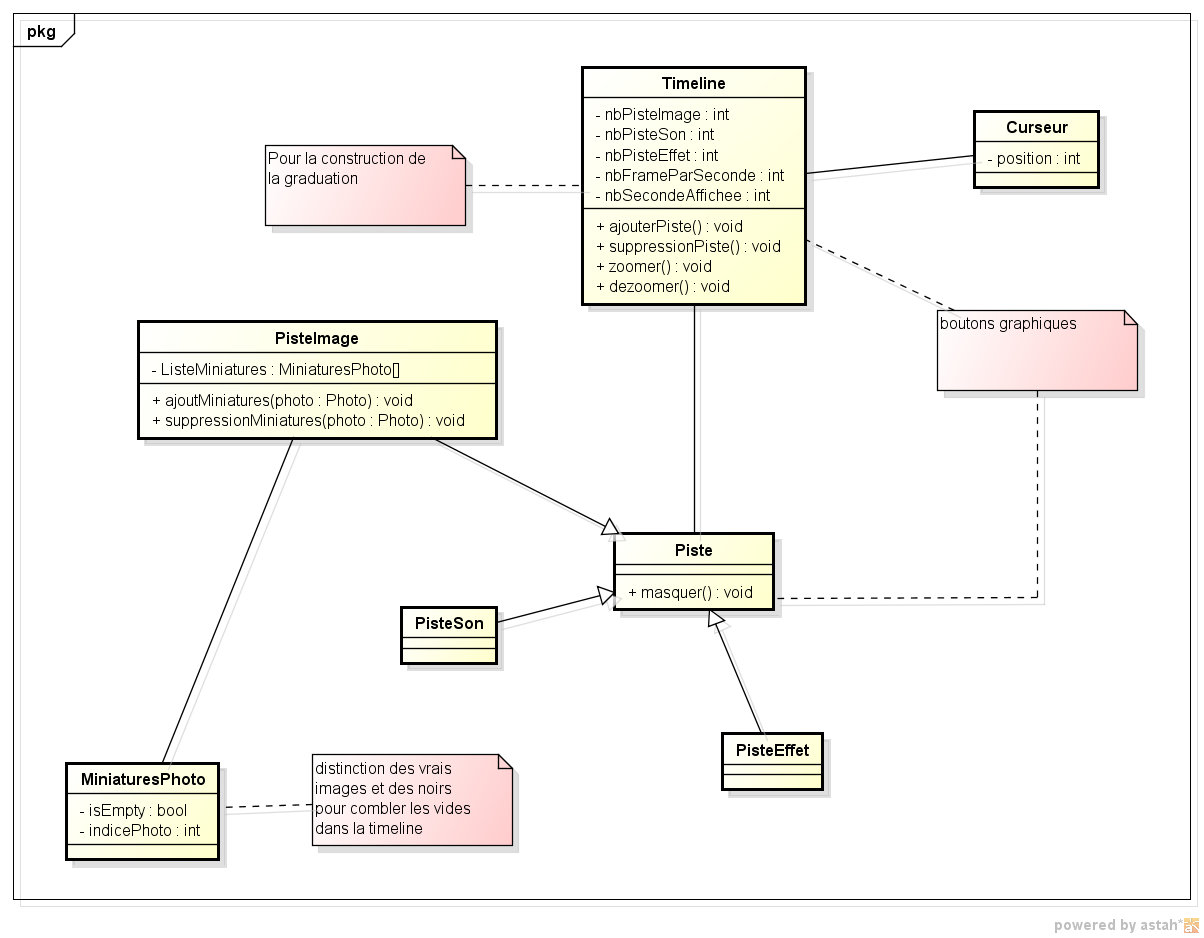
\includegraphics[scale=0.45]{img/diag_class_ex.png}}
   \caption{\label{étiquette} Diagramme de classe du logiciel}
\label{classe}
\end{figure}

Sur ce diagramme, nous avons 5 principaux acteurs.\\
\begin{itemize}
  \item Le Jeu, ou Game, qui représente la partie du jeu. Il fait le lien entre le Joueur (Player) et le Plateau (Board). 
  \item Le Joueur, ou Player, est la classe représentant, comme son nom l'indique, le joueur. C'est lui qui intéragira avec la vue du plateau, et qui donnera des ordres à ses Unités.
  \item Le Plateau, ou Board, contient les cases sur lequel le jeu évolue. Il contient aussi les différentes unités en jeu. Cela permet un accès plus rapide pour le traitement de certaines actions.
  \item Les Cases, ou Tiles, sont les cases, au sens individuel du terme, contenues sur le Plateau. Elle possèdent les Unités qui se trouvent sur elle. Elle hérite 4 autres classes, chacune correspondant au type de terrain associé : Plaine, Désert, Forêt, Montagne.
  \item Les Unités, ou Units, sont les personnages évoluant sur la carte. Les différents peuple sont ici défini comme héritant la classe Unité. Ainsi, on peut surcharger des fonctions, comme le déplacement ou l'attaque, en fonction du peuple de l'Unité : Elf, Orc ou Nain.
\end{itemize}

\subsection{Cas d'utilisations}
Après avoir pensé au logiciel en tant que tel, nous avons réfléchi sur l'interaction que le logiciel aurait avec l'utilisateur. Sur la figure \ref{casdut1}, on peut voir le fonctionnement global du logiciel. Sur la figure \ref{casdut2}, on voit les différentes interactions possibles entre le logiciel et le joueur, lors du tour de ce dernier. 

\begin{figure}[!h] 
\centerline{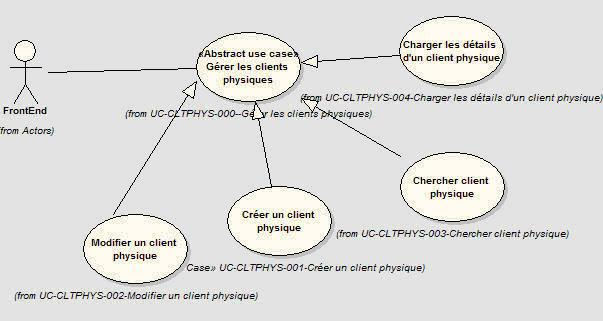
\includegraphics[scale=0.7]{img/diag_cas_dut_ex.jpeg}}
   \caption{\label{étiquette} Diagramme de cas d'utilisations global}
\label{casdut1}
\end{figure}

\begin{figure}[!h] 
\centerline{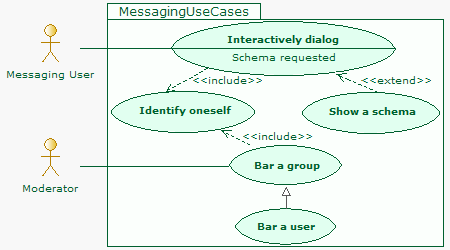
\includegraphics[scale=0.7]{img/diag_cas_dut2_ex.jpeg}}
   \caption{\label{étiquette} Diagramme de cas d'utilisations spécifique}
\label{casdut2}
\end{figure}

\subsection{Déroulement d'un tour}
Le joueur pouvant exécuter de nombreuses actions lors de son tour, nous avons voulu détailler le déroulement d'un tour lambda pour un joueur. Ainsi, nous avons tout d'abord fait un diagramme d'activité permettant une bonne visualisation d'ensemble du tour. On peut voir toutes les actions réalisables, combien de fois le joueur peut les éxecuter, et quelles sont les conditions pour terminer son tour. Le diagramme est représenté sur la figure \ref{activiteTour}

\begin{figure}[!h] 
\centerline{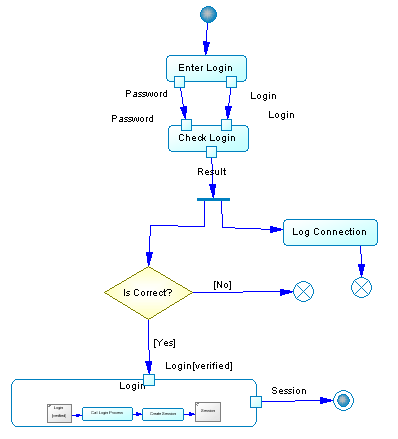
\includegraphics[scale=0.30]{img/activite_tour_ex.png}}
   \caption{\label{étiquette} Diagramme d'activité représentant le déroulement d'un tour pour un joueur}
\label{activiteTour}
\end{figure}

Ensuite, afin d'avoir une vision du tour et des actions du joueur mais en terme de méthodes, de classes et d'interactions, nous avons fait un diagramme de séquence. Il représente le tour d'un joueur ou celui-ci décide de déplacer une de ses unités, puis de terminer son tour. Ce diagramme est représenté sur la figure \ref{sequenceTour}.\\

\begin{figure}[!h] 
\centerline{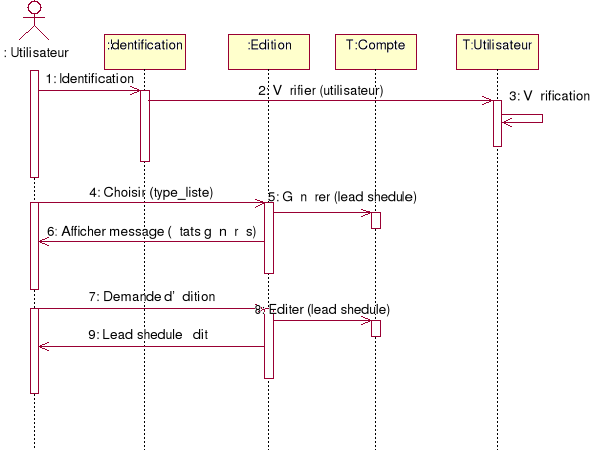
\includegraphics[scale=0.30]{img/sequence_tour_ex.png}}
   \caption{\label{étiquette} Diagramme de séquence représentant le déroulement d'un tour pour un joueur}
\label{sequenceTour}
\end{figure}

\subsection{Déroulement d'une partie}
Après avoir développé un seul tour, nous nous sommes demandés l'interaction entre les tours des joueurs jusqu'à la victoire de l'un d'entre eux. Comme pour le cas d'un seul tour, nous trouvons que les diagrammes de séquences de sont pas adaptés à avoir une vue d'ensemble facilement compréhensible d'un système, c'est pourquoi nous avons fait un autre diagramme d'activité. Il permet de mieux comprendre le fonctionnement d'un tour. Il est représenté en figure \ref{activiteJeu}.\\

\begin{figure}[!h] 
\centerline{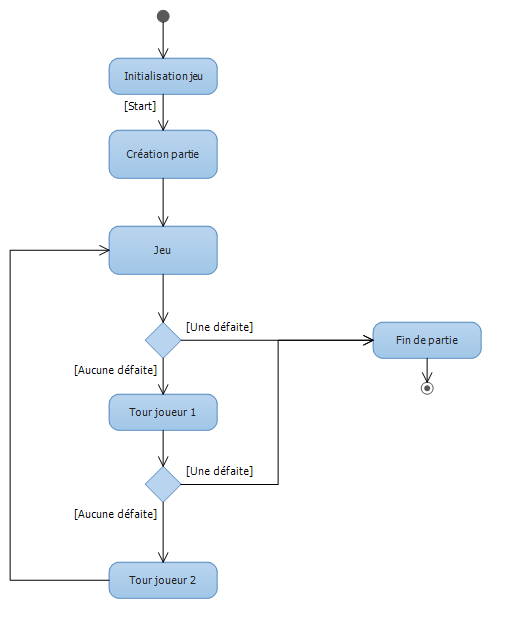
\includegraphics[scale=0.30]{img/activite_jeu_ex.png}}
   \caption{\label{étiquette} Diagramme d'activité représentant le déroulement d'un tour pour un joueur}
\label{activiteJeu}
\end{figure}

Nous avons complété ce diagramme d'activité par un diagramme de séquence, réprésenté en figure \ref{sequenceJeu}, explicitant JE SAIS PU QUEL DIAG ON AVAIT FAIT (DONNER L'EXEMPLE SPECIFIQUE).

\begin{figure}[!h] 
\centerline{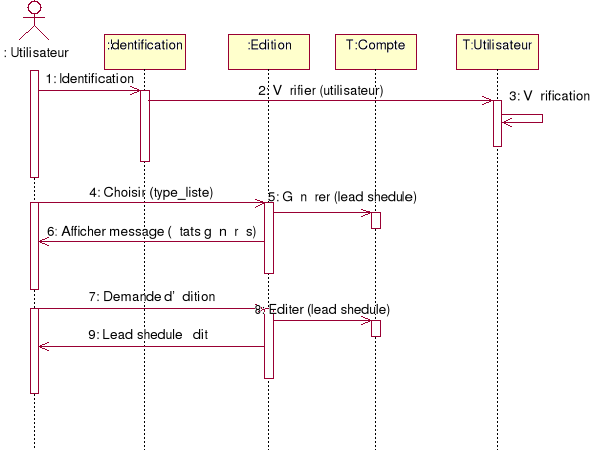
\includegraphics[scale=0.30]{img/sequence_jeu_ex.png}}
   \caption{\label{étiquette} Diagramme de séquence représentant le déroulement d'un tour pour un joueur}
\label{sequenceJeu}
\end{figure}

\subsection{Cycle de vie d'une unité}
Enfin, nous avons voulu nous désintéresser du Jeu et plus nous  au Joueur. Ainsi, nous avons décidé de nous pencher sur le cycle de vie d'une des unités, permettant ainsi d'avoir une vision globale de la durée d'une unité sur le plateau. Nous avons représenté celà sur un diagramme d'état-transitions représenté à la figure \ref{etata}.

\begin{figure}[!h] 
\centerline{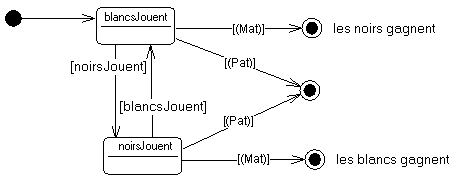
\includegraphics[scale=0.30]{img/etata_ex.png}}
   \caption{\label{étiquette} Diagramme d'état-transition représentant le cycle de vie d'une unité}
\label{etata}
\end{figure}
\newpage

\newpage
\section{conclusion}

\end{document}